\chapter{Datasets}
% OR: \chapter{Data}
\label{cha:data}

\begin{comment}
You will (probably) need to describe and discuss the dataset(s) that you use in your work.
Depending on how much detail is needed and whether you have done any work on the data yourself
(including analysing it, collecting or annotating some of it, or cleaning/preprocessing it),
the data description can possibly be part of the Background chapter, the Related Work chapter,
the Architecture chapter or the Experimental Setup.
The dataset(s) can also be described in a separate chapter, either before or after the chapter on related work.
Note that if you have put some effort of your own into the data, you will need to make sure that the text about it
is part of the ``foreground'' (your own work) rather than the ``background'' (everything done by somebody else), which includes the theoretical
background chapter(s) and the related work.

\textit{Lorem ipsum dolor sit amet, consectetur adipiscing elit. Phasellus pulvinar tempor enim eu hendrerit. Integer consequat ipsum ac erat malesuada, et aliquet dolor gravida. Sed pulvinar vehicula risus id sagittis. Nulla ut nisi ligula. Vestibulum ante ipsum primis in faucibus orci luctus et ultrices posuere cubilia curae; Nullam viverra elit magna, eget interdum enim placerat sed. Duis iaculis non sapien vel tincidunt. Aliquam malesuada molestie mauris ac congue. Nam sit amet felis ex. Nulla convallis tempor lacus eget accumsan. Phasellus arcu velit, pharetra in dolor at, commodo volutpat leo. Praesent nec purus quam. In dignissim vitae sem nec euismod. Maecenas sed feugiat nunc. Cras blandit condimentum libero. Aenean quis efficitur sem.}

\textit{Duis lobortis, mauris a maximus consectetur, sem est interdum justo, eget varius orci augue a tellus. Vestibulum vehicula erat eu eros dignissim, non rhoncus lorem commodo. Mauris et leo vel urna feugiat ornare a ac dolor. Etiam faucibus velit vitae pellentesque ultrices. Pellentesque habitant morbi tristique senectus et netus et malesuada fames ac turpis egestas. Donec facilisis in enim nec fermentum. Vestibulum ante ipsum primis in faucibus orci luctus et ultrices posuere cubilia curae;}

\textit{Maecenas ullamcorper et purus vel facilisis. Pellentesque habitant morbi tristique senectus et netus et malesuada fames ac turpis egestas. Aenean eget diam elit. Vestibulum dolor nunc, porttitor eget porta in, mollis at neque. Phasellus nec tempus diam, non scelerisque orci. Sed tincidunt, lorem a bibendum vehicula, nulla nunc vulputate purus, non viverra sem enim nec est. Aliquam erat volutpat. Praesent in sem tortor. Sed fringilla a nisl et dictum. Nullam faucibus venenatis diam, in sodales magna auctor vel. Suspendisse ornare turpis pulvinar nibh venenatis vulputate.}

\textit{Aliquam eget vulputate tellus. Suspendisse viverra eros sem, eu dapibus diam finibus a. Aenean at lectus eget mi convallis rutrum ut sit amet elit. Curabitur nec nisl mauris. Nullam finibus, elit et vehicula posuere, ante ipsum tristique massa, vitae dictum lorem quam eu est.}

\begin{table}[t!]
    \centering
    \begin{tabular}{l|cccc|c}
        \tabletop
        Dataset   & Normal & Offensive & Hateful & Spam    & Total           \\
        \tablemid
        Original  & 53,790 & 27,037    & 4,948   & 14,024  & \textbf{99,799} \\
        Available & 41,784 & 14,202    & 2,941   & ~~9,372 & \textbf{68,299} \\
        \tablebot
    \end{tabular}
    \caption[The \citeauthor{FountaEA:18} dataset]{The original \citet{FountaEA:18} dataset vs its availability in 2020, given by \citeauthor{Isaksen;Gamback:20}}
    \label{tab:data}
\end{table}

You probably  want a table giving some statistics regarding the data.
As an example, Table~\ref{tab:data} shows a common problem when working with Twitter (X) data:
the authors of a dataset may only provide tweet IDs that other researches can use to retrieve tweets through the Twitter \gls{api};
however, some tweets may for several reasons not be retrievable later on, e.g., since a tweet or the user account behind a tweet may have been deleted.
Here, of $99,799$ tweet IDs provided by \citet{FountaEA:18}, only $68,299$ tweets could actually be retrieved two years later,
as described by \citet{Isaksen;Gamback:20}.

\textit{Morbi viverra ante et tortor faucibus finibus nec sit amet sem. In ultrices, augue sed vestibulum congue, tortor turpis sodales odio, at interdum leo justo non massa. Nunc aliquet, nisl non vestibulum rhoncus, libero tortor laoreet nibh, vel ultricies nunc erat nec nisl. Praesent sed lorem arcu. Sed ultricies, tellus at euismod posuere, felis nibh cursus justo, vitae placerat nisl lorem ut est. Suspendisse sollicitudin sagittis nibh, ac interdum erat hendrerit id. Fusce est mi, semper eget mauris sed, posuere ultrices orci. Aenean nec est eu augue blandit maximus. Morbi ut nisl at metus condimentum tincidunt nec consectetur nibh. Phasellus eleifend dapibus elit ut cursus. Donec lacinia turpis a justo dignissim, sit amet venenatis libero pellentesque. Orci varius natoque penatibus et magnis dis parturient montes, nascetur ridiculus mus.}
\end{comment}

With the interest of investigating the ability of a \gls{acr:llm}-based system to perform geospatial analysis, relevant datasets should be accessible to said system. \Autosectionref{sec:data-sources} provides a description of the datasets used in the experiments. Furthermore, it was decided to explore different access channels to this data. \Autosectionref{sec:data-access} elaborates on this.

\section{Data Sources}
\label{sec:data-sources}

\begin{comment}
A total of eight datasets were used in the experiments. All datasets were downloaded through Geonorge\footnote{\url{https://geonorge.no}}, a webpage administered by The Norwegian Mapping Authority that serves as a portal to a large catalogue of Norwegian geographical data. The datasets were selected to provide a diverse pool of geographical data to perform analysis upon. \autoref{tbl:datasets} shows the datasets used along with a description.


\begin{table}[htbp]
    \centering
    \caption{Datasets used in experiments}
    \label{tbl:datasets}
    \begin{tabularx}{\textwidth}{p{3cm}|X}
        \toprule
        \textbf{Dataset}                          & \textbf{Description}                                                                                                                                                                                                                                                                              \\
        \midrule
        AR50 - Land Use Map                       & A nationwide dataset that displays main types of land use adapted for use in scales from 1:20,000 to 1:100,000.                                                                                                                                                                                   \\
        \midrule
        Strategic Noise Mapping from Road Traffic & The strategic noise mapping shows the noise situation from road traffic at the turn of the year 2016/2017 for the largest urban areas in the country and in addition along national and county roads where more than 8,200 vehicles pass per day.                                                 \\
        \midrule
        Elveg 2.0 - Road Network                  & A road network dataset that includes all drivable roads that are longer than 50 meters, or part of a network, as well as pedestrian and bicycle paths and bicycle paths represented as road link geometry.                                                                                        \\
        \midrule
        Cadastrial Register - Building Points     & The Matrikkelen-Building point dataset contains a small excerpt of the building information registered in the Matrikkelen, Norway's official register of real property, including buildings. The dataset contains representation points, building type, building number, current building status. \\
        \midrule
        Outdoor Recreation Areas                  & The purpose of the dataset is to provide an overview of areas that are important for the public's outdoor life, and it should be easy to account for which assessments and criteria have been the basis for the work and the final product.                                                       \\
        \midrule
        Cultural Monuments - Protected Buildings  & Buildings and churches that are automatically, decision, regulation, or temporarily protected under law and churches that have the status as listed.                                                                                                                                              \\
        \midrule
        Flood Zones                               & Flood zones show areas that are flooded by different flood sizes (recurrence interval). Flood zones are prepared for 20-, 200-, and 1000-year floods.                                                                                                                                             \\
        \midrule
        Quick Clay Zones                          & Provides an overview of zones with potential danger (precautionary areas) for major quick clay landslides.                                                                                                                                                                                        \\
        \bottomrule
    \end{tabularx}
\end{table}

\end{comment}

A total of eighteen datasets were used in the experiments. The data was downloaded from Geofabrik's website\footnote{\url{https://download.geofabrik.de/europe/norway.html}}. Geofabrik --- German for \enquote{geo factory} --- is a company that \enquote{extract, select, and process free geodata}. They have gathered data from OpenStreetMap and published them as a collection of shapefiles, dividing them into categories such as \enquote{places of worship}, \enquote{points of interest}, and \enquote{traffic}. Data can be downloaded for different regions of the world, and for experiments conducted in this thesis, data for Norway was used. \autoref{tbl:datasets} in \autoref{app:datasets} lists all datasets used, along with a short description of their contents. Common for all datasets are their \emph{fclass} attribute, which is short for \emph{feature class}. Some datasets have additional attributes, such as the \emph{maxspeed} attribute in the road data and the \emph{type} attribute in the building data. \autoref{fig:datasets-trondheim} shows a plot containing four selected datasets, constrained to a bounding box of Trondheim. The plot was created by GeoGPT.

\begin{figure}
    \centering
    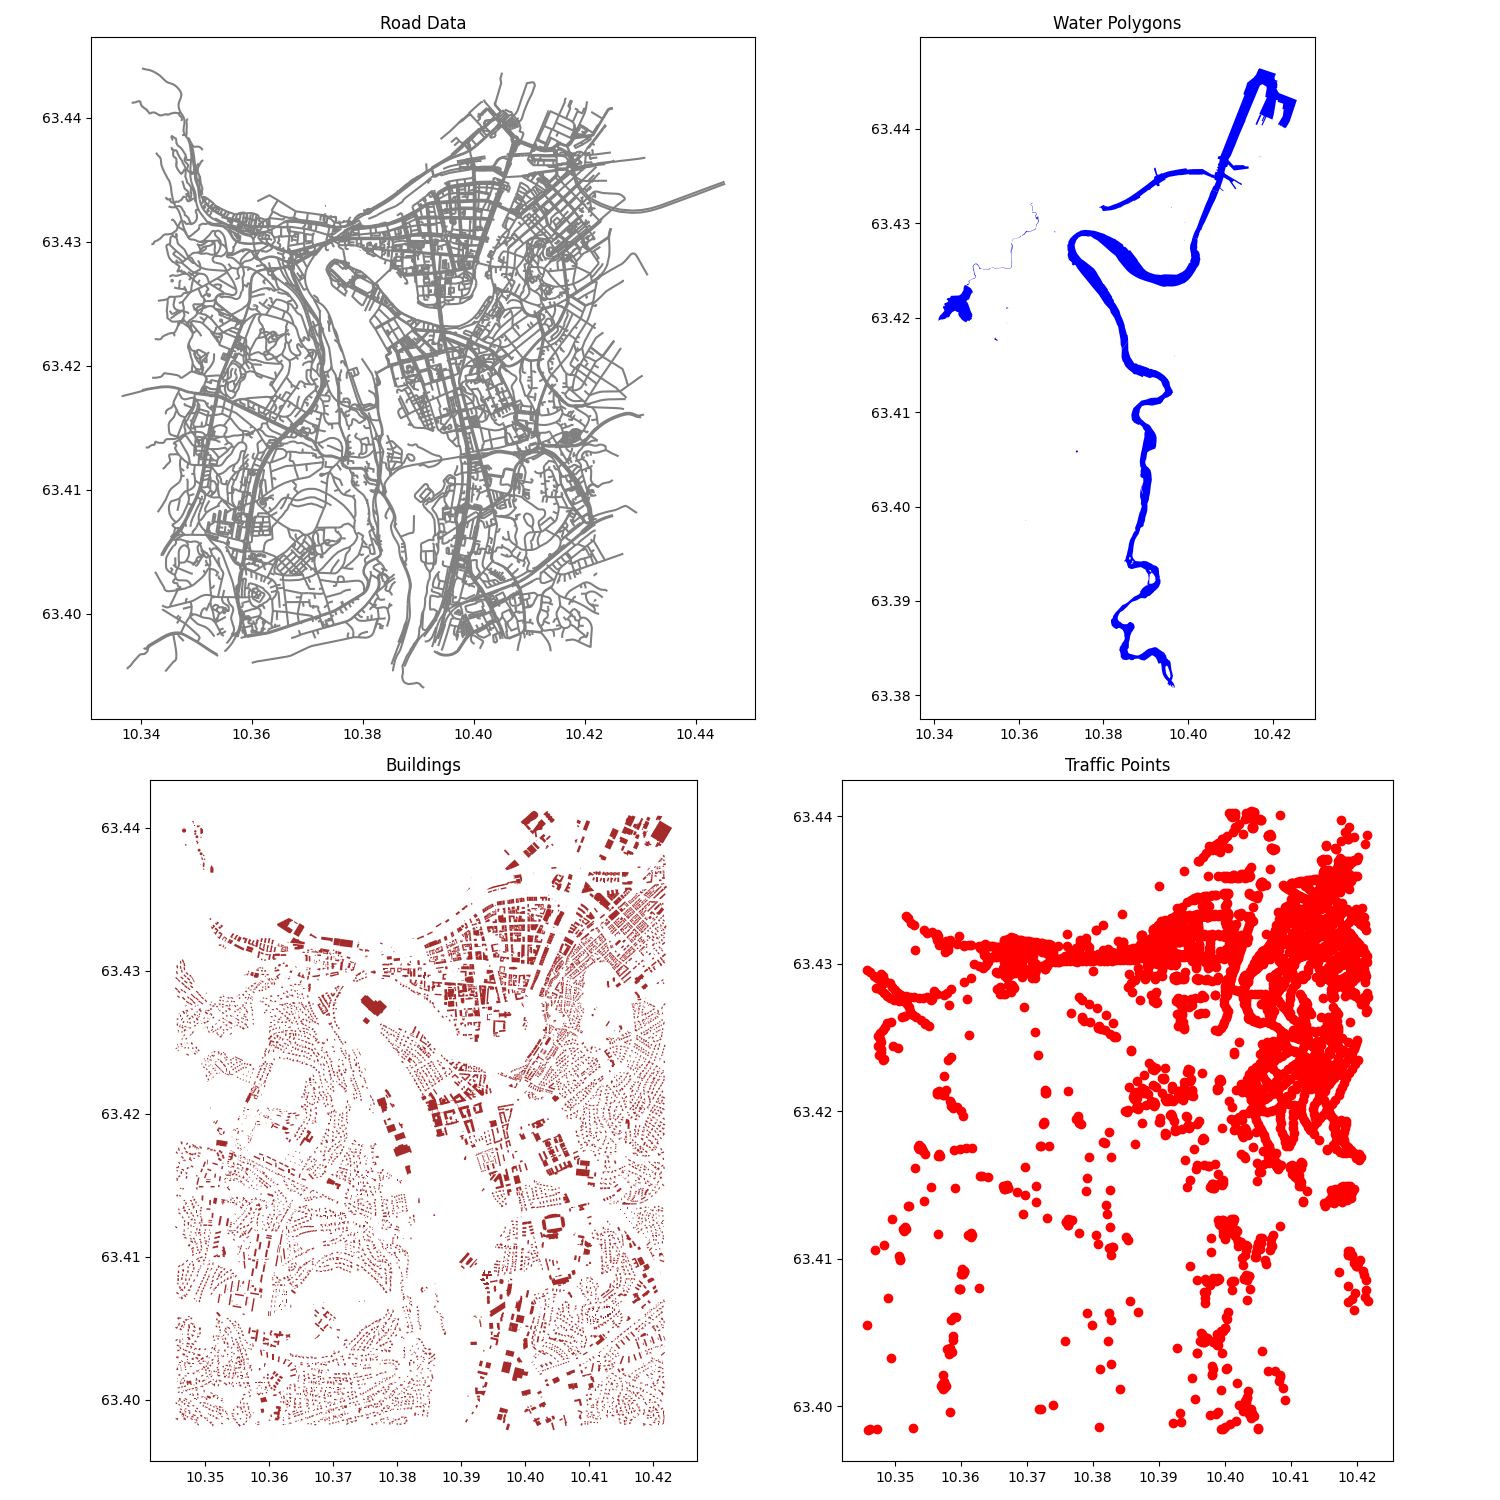
\includegraphics[width=\textwidth]{trondheim_datasets.png}
    \label{fig:datasets-trondheim}
    \caption{A plot of four selected datasets constrained to a polygon of Trondheim}
\end{figure}

\section{Data Access}
\label{sec:data-access}

While leading \glspl{acr:llm} are trained on increasingly large corpora, they are still only as familiar with a topic as the extent to which the training data exposes it to said topic. For instance, many \glspl{acr:llm} are trained specifically to generate Python code, and are therefore fed with a vast number of Python code examples during training in the hopes of improving its performance on benchmarks like the \gls{acr:mbpp} benchmark \citep{austinProgramSynthesisLarge2021}. As it is unlikely that the training data is evenly distributed among many different topics, it is useful to get familiarized with a model's capabilities in the areas of interest for a particular use case. In the case of an \acrshort{acr:llm}-powered \acrshort{acr:gis} agent that should be capable of performing geospatial analyses, it is useful to know what data formats such an agent is most comfortable to understand and work with. The upcoming experiments therefore seek to benchmark model performance on three different data access methods.

The first method of presentation is to have the files from \autoref{sec:data-sources} remain untouched. The files are stored locally on the computer on which the experiments are conducted and GeoGPT, which runs on the same computer, is able to interact with the data through the code that it generates. These files are stored on a location unknown to GeoGPT but are made available through a working directory --- which location \textit{is} known to GeoGPT --- through symbolic links to the unknown location of the actual files. \autoref{code:python-munkegata-bbox} in the \autoref{cha:experiments} shows how GeoGPT is able to use Python code it has generated to load road data, perform intersection with a bounding box, and writing the result to a new file in the working directory.

The second method used is to load the data into a spatial \acrshort{acr:sql} database and provide the model with database schemas that can be used to generate queries. The datasets were uploaded to a Dockerized PostGIS database using QGIS's DB Manager plugin.

The third method for data access is to use the \acrshort{acr:ogc} \acrshort{acr:api} Features standard. In essense, this methods serves the data stored in the PostGIS database as a web server that allows consumers of the \acrshort{acr:api} to download the data over \acrshort{acr:http} as GeoJSON.

\glsresetall
